\documentclass[11pt, a4paper]{article}

% -- PACKAGES -- 
% Document structure and impagination
\usepackage[margin=3cm]{geometry}
\usepackage{setspace}

% Allows colors usage
\usepackage[dvipsnames]{xcolor} 

% Images management
\usepackage{graphicx}

% Tables 
\usepackage{tabularx}
\usepackage{multirow}
\usepackage{colortbl}

% Hyperlinks
\usepackage[hidelinks]{hyperref}

% Allows math formulas usage
\usepackage{mathtools}

% PDFs
\usepackage{pdfpages}

% Captions
\usepackage{subcaption}
\usepackage{booktabs}
\usepackage{float} 

% Code
\usepackage{listings}

% -- SETTINGS --
% Captions Settings
\DeclareCaptionFormat{custom} {
    \textbf{#1}\\
	\vspace*{4pt}
	\small{#3}
}
\captionsetup{format=custom}

% Tables formatting
\setlength{\tabcolsep}{0.5em}

%% -- COLORS --
% Colors used in the document 
\definecolor{unicefBlue}{HTML}{1CABE2}
\definecolor{unicefRed}{HTML}{D72929}
\definecolor{unicefOrange}{HTML}{EA8A2D}
\definecolor{unicefGreen}{HTML}{1A8724}
\definecolor{unicefGray}{HTML}{8B8B8B}

% -- DOCUMENT --
% Document structure
\begin{document}
\pagenumbering{gobble}

% Document cover
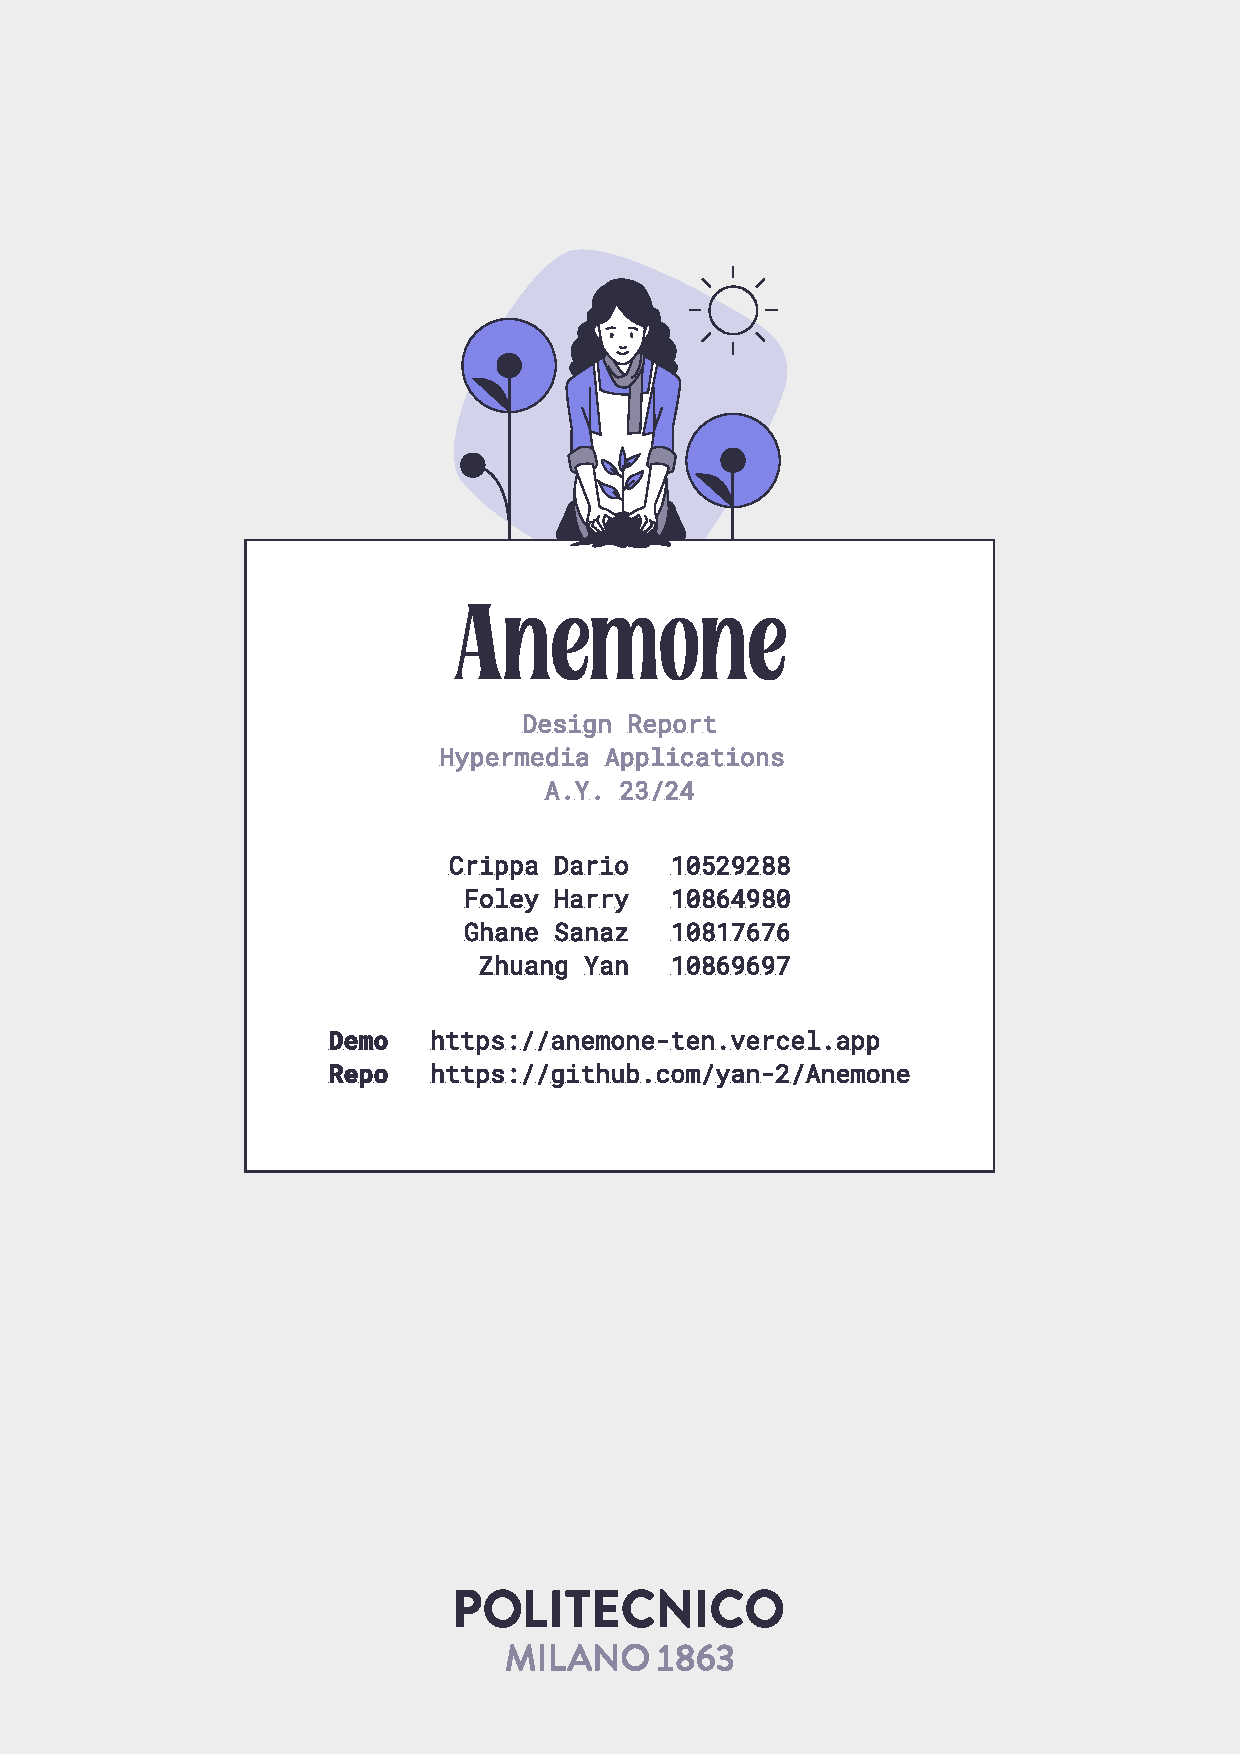
\includepdf{Resources/cover.pdf}

% Table of contents
\tableofcontents

% -- CHAPTERS -- 
% Abstract
% Document abstract 
\pagenumbering{arabic}
\section{Abstract}
The aim of this document is to carry out a usability evaluation of the website
\begin{center}
    \url{https://www.unicef.org}
\end{center}
We can distinguish two main areas: inspection and user testing. 
\subsection{Inspection}
For the site inspection, we selected twelve heuristics from the MiLe set in addition to those from Nielsen.
Each team member performed individual analyses and the results were discussed together to identify the most critical issues.
We chose not to average the results of the individual scores, recognising that details missed in the individual reviews could significantly alter the previously provided scores.
The joint assessment did not reveal any significant critical issues at the site; however, there is still considerable room for improvement in certain areas.
In particular, our evaluation revealed a prevailing sense of disorientation in navigation, coupled with a lack of consistency.

\subsection{Testing}
To streamline the tests, we created a series of high-level tasks without going into detailed instructions on how to perform them. 
We meticulously recorded the time taken by each participant to complete each task, and then set thresholds to classify test results as either successful or unsuccessful. 
For logistical reasons, we conducted some tests remotely rather than in person.
Participants were unable to interact with us in any way. Our focus was solely on gathering personal and non-personal feedback on the usability of the site.
The majority of the tests were conducted using a PC, with some testers specifically tasked to evaluate the site from a mobile device.
The tests confirmed many of our personal impressions and shed light on some aspects we had not previously considered, such as the poor experience of using the site from a mobile device.
% Content
\section{Conceptual Design}
\subsection{CIDM Diagram}
The general structure of the website was defined using the C-IDM in the large notation. 
This method ensures that particular attention is paid to the relations among topics within groups and their cardinality, 
which is defined as the expected minimum and maximum number of instances of a topic or relation.

% CIDM Image

A detailed preview of the page content was crafted using the C-IDM in the small notation, presented as Content Tables.

% Contacts
\begin{table}[htp!]
    \centering
    \begin{tabular}{ |l|l| }
        \hline
        \rowcolor{anemoneBlue}
        \multicolumn{2}{ |l| }{\color{white}{\textbf{Topic : Contacts}}}\\
        \hline
        \textbf{Title} & \texttt{Text} \color{anemoneGray}{Contacts}\\
        \hline
        \textbf{Subtitle} & \texttt{Text} \color{anemoneGray}{max 64 chars}\\
        \hline
        \textbf{Phone Number} & \texttt{Text} \color{anemoneGray}{max 64 chars}\\
        \hline
        \textbf{Email} & \texttt{Text} \color{anemoneGray}{max 64 chars}\\
        \hline
        \textbf{Address} & \texttt{Text} \color{anemoneGray}{max 128 chars}\\
        \hline
        \textbf{Map} & \texttt{Interactive Map}\\
        \hline
    \end{tabular}
\end{table}

% Person
\begin{table}[htp!]
    \centering
    \begin{tabular}{ |l|l| }
        \hline
        \rowcolor{anemoneBlue}
        \multicolumn{2}{ |l| }{\color{white}{\textbf{Kinf of Topic : Person}}}\\
        \hline
        \textbf{Name} & \texttt{Text (max 64 chars)}\\
        \hline
        \textbf{Picture of Person} & \texttt{Image} \\
        \hline
        \textbf{CV} & \texttt{Text (max 200 words)}\\
        \hline
        \textbf{Activities Responsible for} & \texttt{List of [Links(Activity Name)]}\\
        \hline
    \end{tabular}
\end{table}

% Project
\begin{table}[htp!]
    \centering
    \begin{tabular}{ |l|l| }
        \hline
        \rowcolor{anemoneBlue}
        \multicolumn{2}{ |l| }{\color{white}{\textbf{Kinf of Topic : Project}}}\\
        \hline
        \textbf{Project Name} & \texttt{Text (max 64 chars)}\\
        \hline
        \textbf{Picture of Project} & \texttt{Image} \\
        \hline
        \textbf{Short Description} & \texttt{Text (max 200 words)}\\
        \hline
        \textbf{Person Responsible} & \texttt{Link (Person's Name)}\\
        \hline
    \end{tabular}
\end{table}

% Service
\begin{table}[htp!]
    \centering
    \begin{tabular}{ |l|l| }
        \hline
        \rowcolor{anemoneBlue}
        \multicolumn{2}{ |l| }{\color{white}{\textbf{Kinf of Topic : Service}}}\\
        \hline
        \textbf{Service Name} & \texttt{Text (max 64 chars)}\\
        \hline
        \textbf{Picture of Service} & \texttt{Image} \\
        \hline
        \textbf{Short Description} & \texttt{Text (max 100 words)}\\
        \hline
        \textbf{Key Benefits} & \texttt{Text (max 100 words)}\\
        \hline
        \textbf{Person Responsible} & \texttt{Link (Person's Name)}\\
        \hline
        \textbf{Practical Information} & \texttt{Text (max 100 words)}\\
        \hline
        \textbf{Testimonial} & \texttt{Text (max 100 words)}\\
        \hline
    \end{tabular}
\end{table}

% Centre
\begin{table}[htp!]
    \centering
    \begin{tabular}{ |l|l| }
        \hline
        \rowcolor{anemoneBlue}
        \multicolumn{2}{ |l| }{\color{white}{\textbf{Topic : Centre}}}\\
        \hline
        \textbf{Title} & \texttt{Text (max 64 chars)}\\
        \hline
        \textbf{Description} & \texttt{Text (max 100 words)}\\
        \hline
        \textbf{Practical Information} & \texttt{Text (max 100 words)}\\
        \hline
        \textbf{Map} & \texttt{Interactive Map}\\
        \hline
    \end{tabular}
\end{table}



% FAQ
\begin{table}[htp!]
    \centering
    \begin{tabular}{ |l|l| }
        \hline
        \rowcolor{anemoneBlue}
        \multicolumn{2}{ |l| }{\color{white}{\textbf{Topic : FAQ}}}\\
        \hline
        \textbf{Title} & \texttt{Text} \color{anemoneGray}{max 32 chars}\\
        \hline
        \textbf{Description} & \texttt{Text} \color{anemoneGray}{max 576 chars}\\
        \hline
    \end{tabular}
\end{table}

% All People
\begin{table}[htp!]
    \centering
    \begin{tabular}{ |l|l| }
        \hline
        \rowcolor{anemoneBlue}
        \multicolumn{2}{ |l| }{\color{white}{\textbf{Group : People}}}\\
        \hline
        \textbf{Title} & \texttt{Text (max 64 chars)}\\
        \hline
        \textbf{Description} & \texttt{Text (max 64 chars)}\\
        \hline
        \textbf{Persons} & \texttt{List of [Name, Profile Image, Role]}\\
        \hline
    \end{tabular}
\end{table}

% All Projects
\begin{table}[htp!]
    \centering
    \begin{tabular}{ |l|l| }
        \hline
        \rowcolor{anemoneBlue}
        \multicolumn{2}{ |l| }{\color{white}{\textbf{Group : Projects}}}\\
        \hline
        \textbf{Title} & \texttt{Text (max 64 chars)}\\
        \hline
        \textbf{Description} & \texttt{Text (max 64 chars)}\\
        \hline
        \textbf{Projects} & \texttt{List of [Name, Project Image, Description]}\\
        \hline
    \end{tabular}
\end{table}

% All Services
\begin{table}[htp!]
    \centering
    \begin{tabular}{ |l|l| }
        \hline
        \rowcolor{anemoneBlue}
        \multicolumn{2}{ |l| }{\color{white}{\textbf{Group : Services}}}\\
        \hline
        \textbf{Title} & \texttt{Text (max 64 chars)}\\
        \hline
        \textbf{Description} & \texttt{Text (max 64 chars)}\\
        \hline
        \textbf{Services} & \texttt{List of [Name, Service Image, Description]}\\
        \hline
    \end{tabular}
\end{table}

\subsection{Mapping}
The content tables in the preceding section have the same name as the pages they represent. 
The following section presents the manner in which they are connected.

\subsection{PIDM Diagram}
The P-IDM notation was used to define the navigation capabilities of the website. 
This resulted in a tree-like structure with the homepage as the root, from which every page is eventually reachable.

% PIDM Image
\include{Chapters/visual.tex}
\include{Chapters/interactions.tex}
\include{Chapters/database.tex}

\end{document}
